% !TEX program = pdflatex
% =============================================================================
%  PKU Technical Report Template -- Demo / Example Document
%
%  This file demonstrates how to use the PKU Technical Report template
%  (style.cls) for a survey paper. It includes:
%    - Title, authors, affiliations
%    - Abstract with project links
%    - Full-width overview figure
%    - Section structure with subsections
%    - Tables, algorithms, and colored boxes
%    - Bibliography
%
%  Compile with:  latexmk -pdf demo.tex
% =============================================================================
\documentclass[]{style}

\usepackage[toc,page,header]{appendix}
\usepackage{enumitem}

% For flexible citation formats (author-year, numeric)
\usepackage{natbib}

% For UTF-8 encoded CJK (Chinese, Japanese, Korean) characters
\usepackage{CJKutf8}

% enables \newcommandx
\usepackage{xargs}

% for creating todo notes
\usepackage{todonotes}

% for table \multirow
\usepackage{multirow}


% for \cref
\usepackage{cleveref}

\usepackage{amsmath}
\usepackage{dsfont}

% % using itemize
% \usepackage{enumerate}



% \usepackage{svg}  % needs Inkscape + pdflatex --shell-escape; uncomment only if you use \includesvg

\usepackage{mathrsfs}
\usepackage{adjustbox}
\usepackage{multirow}
\usepackage{multicol}
\usepackage{tcolorbox}
\usepackage{changepage}
\usepackage{enumitem}
\usepackage{graphicx}
\usepackage{amssymb}
\usepackage{xcolor}
\usepackage{float}
\usepackage{multirow}
\usepackage{threeparttable}
\usepackage{graphicx}
\usepackage{subcaption}
\usepackage{algorithm}
\usepackage{algpseudocode}
\usepackage{wrapfig}
\usepackage[table]{xcolor}  % loads xcolor with table support
\usepackage{colortbl}       % gives \columncolor, \rowcolor
\usepackage{tabularx} % Add to your preamble
\usepackage{makecell} % Add to your preamble
\usepackage[dvipsnames]{xcolor}

\newcolumntype{g}{>{\columncolor{gray!10}}c} % gray background
\newcommand{\KVSet}{\mathbf{KV}}
\newcommand{\ModelOuput}{\mathbf{X}_{\theta}}
\newcommand{\KVOutput}{\mathbf{kv}}

\definecolor{catgray}{gray}{0.9}
\definecolor{skyblue}{rgb}{0.53,0.81,0.92} % sky blue

% make it look transparent by mixing with white
\colorlet{skyblue!30}{skyblue!30!white} % 30% skyblue, 70% white

\definecolor{customblue}{RGB}{70,130,180}  % This is equivalent to rgb(70,130,180)

\newtcolorbox{evolbox}[2][]{%
  enhanced,
  % colframe=blue!70!black,
  colframe=customblue,
  colback=white,
  coltitle=white,
  rounded corners,
  boxrule=1pt,
  titlerule=0pt,
  toptitle=1mm,
  bottomtitle=1mm,
  fonttitle=\bfseries,
  % title=#3,
  % fontupper=\boxcontentfont\fontsize{10pt}{12pt}\selectfont,
  width=#2\textwidth, % This takes the second parameter as the width fraction
  % Applying the custom font with size
  % left=1mm, % Reduced left padding
  % right=1mm, % Reduced right padding
  % top=1mm, % Reduced top padding
  % bottom=1mm, % Reduced bottom padding
  #1
}
%%%%%%%%%%%%%%%%%%%%%%%%%%%%%%%%%%%%

\usepackage{minitoc}
\usepackage{url}

% cvpr packages
\PassOptionsToPackage{table,xcdraw}{xcolor}
\usepackage{titletoc}
\usepackage{placeins}
% checkmark / cross symbols for tables
\usepackage{pifont}

% \definecolor{cvprblue}{rgb}{0.21,0.49,0.74}
% \usepackage[pagebackref,breaklinks,colorlinks,allcolors=cvprblue]{hyperref}
\definecolor{RowBlue}{HTML}{E9F2FB}
\definecolor{RowRed}{HTML}{F9EAEA}
\definecolor{Top1}{HTML}{50DB4B} % dark green
\definecolor{Top2}{HTML}{A5FFA2} % medium green
\definecolor{Top3}{HTML}{D9FFD9} % light green
\definecolor{Sub1}{HTML}{EAB8B8}
\definecolor{Sub2}{HTML}{E4E4E4}
\newcommand{\cmark}{\textcolor{green!60!black}{\checkmark}}
\newcommand{\xmark}{\textcolor{red!70!black}{\ding{55}}}

\newcommand{\reviewnote}[1]{{\textcolor{cyan}{[NOTE: #1]}}}
\newcommand{\myparagraph}[1]{\textbf{#1}\hspace{1.8ex}}

\renewcommand{\emph}[1]{\textit{#1}}

\setlength{\cftbeforesubsecskip}{1.5pt}

%%%%%%%%%%%%%%%%%%%% Title / Authors / Affiliation %%%%%%%%%%%%%%%%%%%%

\title{Beyond OCR: A Survey of Document Intelligence\\from Structured Perception to Multimodal Question Answering}

\author{
  JiaShu Yang\texorpdfstring{$^{1}$}{} \hspace{0.1cm}
  Chi Zhang\texorpdfstring{$^{1}$}{} \hspace{0.1cm}
  Xingyu Qi\texorpdfstring{$^{1}$}{} \hspace{0.1cm}
  Ning Zhang\texorpdfstring{$^{1}$}{} \hspace{0.1cm}
  Jie Wu\texorpdfstring{$^{1}$}{} \hspace{0.1cm}
  Lingxu Chen\texorpdfstring{$^{1}$}{} \hspace{0.1cm}
  Jiani Guo\texorpdfstring{$^{1}$}{}
}

\makeatletter
\g@addto@macro\authorlist{\\[3mm]
  {\authorfont\sffamily Document Intelligence Research Group\texorpdfstring{$^{}$}{}}%
}
\makeatother

\affiliation[]{Peking University}

%%%%%%%%%%%%%%%%%%%% Abstract %%%%%%%%%%%%%%%%%%%%

\abstract{%
Documents (paper media, images, or electronic files containing textual and graphical information) are ubiquitous in daily office work, online dissemination, and governmental and enterprise workflows; automatically parsing, retrieving, and supporting decision-making based on their content constitutes a core requirement of Document Intelligence.

Following this evolution, this paper organizes the survey in the order of ``perception first, then reasoning, and finally end-to-end unified modeling,'' and aligns evaluation suites with methodological lineages. Part~I (Document Layout Analysis and OCR) focuses on layout parsing starting from page geometry. Part~II (Document Understanding and Question Answering) systematically summarizes three mainstream scenarios built on structured inputs.
}

%%%%%%%%%%%%%%%%%%%% Header links %%%%%%%%%%%%%%%%%%%%
\checkdata[
\raisebox{-0.2em}{
\includegraphics[width=0.025\linewidth]{figs/icons/globe.png}}~~Project Page]{\href{https://github.com/your-org/document-intelligence-survey}{\texttt{https://github.com/your-org/document-intelligence-survey}}
\\[-1.5ex]}

\checkdata[
\raisebox{-0.2em}{
\includegraphics[width=0.025\linewidth]{figs/icons/github.png}}~~Code Repository]{\href{https://github.com/your-org/document-intelligence-survey}{\texttt{https://github.com/your-org/document-intelligence-survey}}
\\[-1.7ex]}

\checkdata[
\raisebox{-0.2em}{
\includegraphics[width=0.025\linewidth]{figs/icons/mail.png}}~~Correspondence]{\href{mailto:jiashuyang@pku.edu.cn}{\texttt{jiashuyang@pku.edu.cn}}
\\[-1.7ex]}


\begin{document}
\maketitle

%%--------------------------------------------------------------------
%%  Full-width overview figure (spanning both columns)
%%--------------------------------------------------------------------
\begin{figure*}[t]
\centering
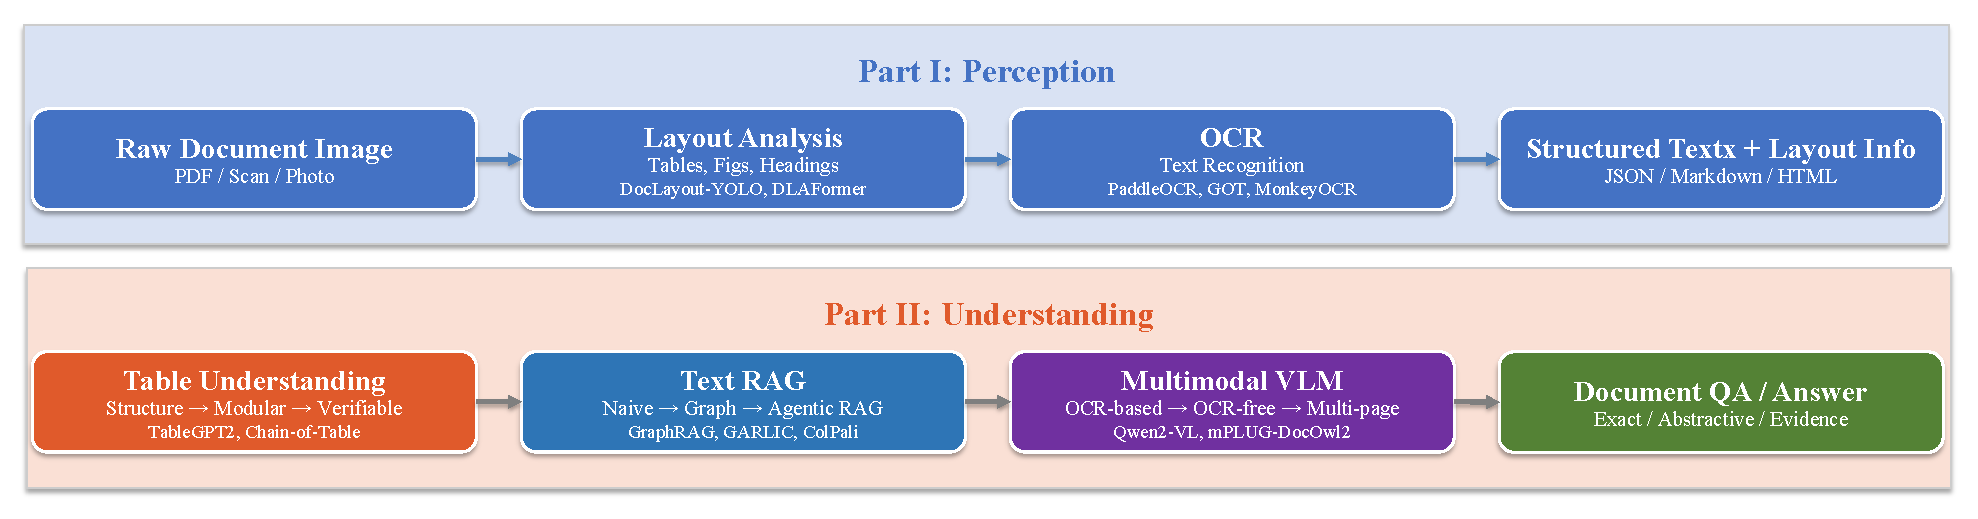
\includegraphics[width=\textwidth]{figs/fig01.pdf}
\caption{Overview of the Document Intelligence pipeline: Part~I (Perception) covers layout analysis and OCR, producing structured text and layout; Part~II (Understanding) includes three parallel branches---table understanding, text RAG, and multimodal VLM---each converging on the final Document QA output.}
\label{fig:pipeline_overview}
\end{figure*}


%%--------------------------------------------------------------------
%%  Section 1: Introduction
%%--------------------------------------------------------------------
\section{Introduction}
\label{sec:intro}

Documents are fundamental carriers of human knowledge, encompassing a vast array of formats including academic papers, business reports, legal contracts, medical records, and financial statements. The automatic understanding of these documents---extracting structured information, answering questions, and supporting decision-making---has long been a central challenge in artificial intelligence.

The document processing pipeline traditionally follows a two-stage paradigm: \textit{perception} followed by \textit{reasoning}. In the perception stage, documents are first converted into machine-readable representations through Optical Character Recognition (OCR) and layout analysis. The reasoning stage then operates on these structured representations to perform higher-level tasks.

\subsection{Scope and Contributions}

This survey provides a comprehensive review of document intelligence research, organized around the core pipeline illustrated in \cref{fig:pipeline_overview}. Our contributions are threefold:

\begin{enumerate}[leftmargin=*]
    \item \textbf{Structured Taxonomy}: We present a systematic organization of the field along two dimensions---perception and reasoning.
    \item \textbf{Technical Depth}: For each research direction, we trace the evolution from early heuristic methods through deep learning innovations to contemporary LLM/VLM-based approaches.
    \item \textbf{Evaluation Perspective}: We provide a comprehensive overview of benchmarks spanning single-page to multi-page documents.
\end{enumerate}


%%--------------------------------------------------------------------
%%  Section 2: Layout Analysis and OCR
%%--------------------------------------------------------------------
\section{Document Layout Analysis and OCR}
\label{sec:layout_ocr}

This section covers the perception stage of document intelligence, focusing on two fundamental tasks: \textbf{Document Layout Analysis} and \textbf{Optical Character Recognition}.

\subsection{Document Layout Analysis}

Document layout analysis has evolved from rule-based heuristic methods to sophisticated deep learning approaches that jointly model visual appearance, textual content, and spatial relationships.

\subsubsection{Geometric Structure Detection}

Early approaches treated layout analysis as a computer vision problem focused on detecting and classifying document elements based on their geometric and visual properties. The deep learning era brought significant advances through the adoption of object detection architectures.

\subsubsection{Layout-Aware Representation Learning}

Beyond pure visual detection, modern approaches integrate layout information directly into representation learning. LayoutLM pioneered the joint modeling of text content and 2D positional information within the Transformer pre-training framework.

\begin{figure*}[t]
\centering
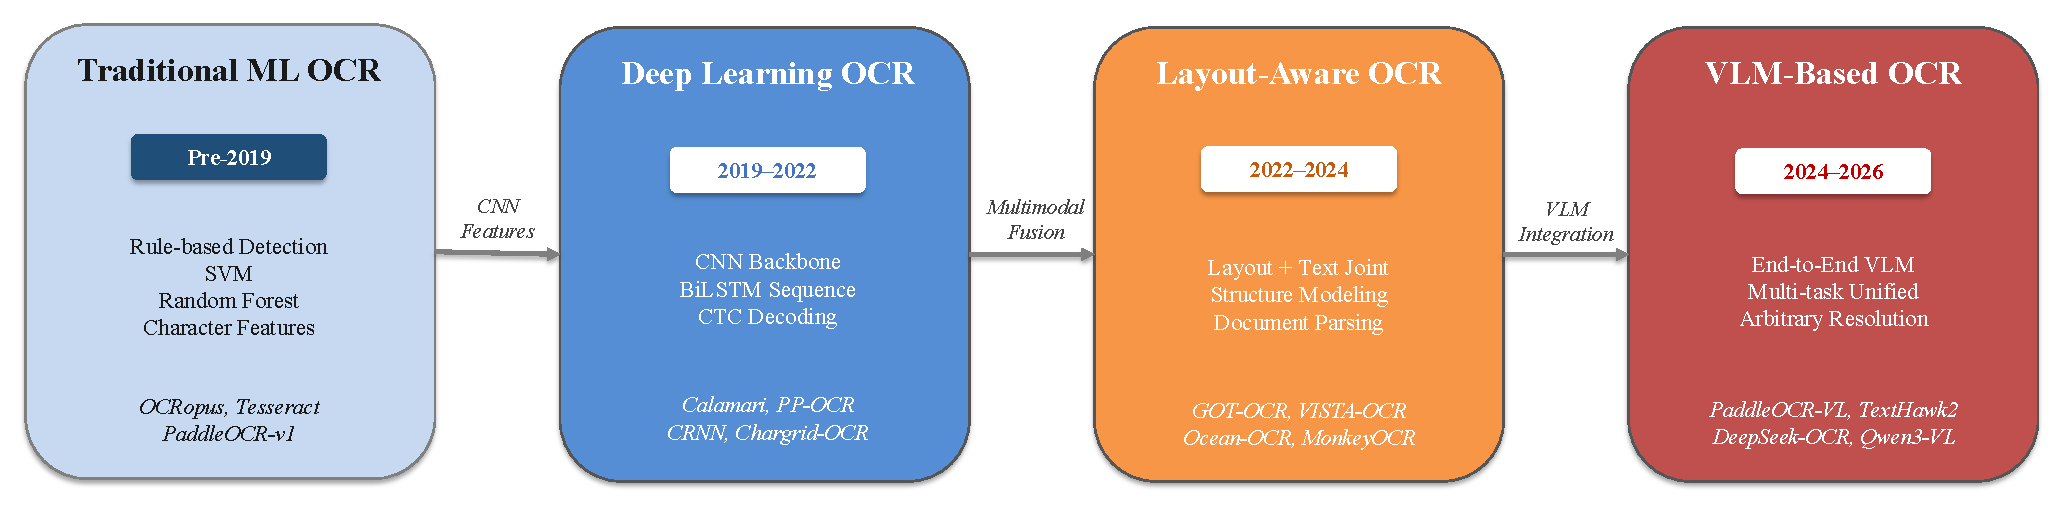
\includegraphics[width=0.95\textwidth]{figs/fig02.pdf}
\caption{Four-stage evolution of optical character recognition technology: from rule-based Traditional Machine Learning methods, through Deep Learning approaches, to Layout-Aware OCR, and finally to Vision-Language Model-based OCR.}
\label{fig:ocr_evolution}
\end{figure*}

\subsection{Optical Character Recognition}

OCR technology has undergone a four-stage evolution (\cref{fig:ocr_evolution}): from rule-based traditional methods, through deep learning approaches with CNN-BiLSTM-CTC pipelines, to Layout-Aware OCR with joint structure modeling, and finally to Vision-Language Model-based OCR.


%%--------------------------------------------------------------------
%%  Section 3: Table Understanding
%%--------------------------------------------------------------------
\section{Table Understanding and Question Answering}
\label{sec:table}

Tables present unique challenges for document understanding: they encode structured relational data with implicit row-column dependencies, header hierarchies, and cell-level semantics that are easily lost when linearized into text.

\subsection{Structure-Aware and Table Semantic Modeling}

Early research recognized that simple table linearization weakened the ability to model row-column relationships and cell dependencies. Intermediate pre-training approaches significantly improved table understanding capabilities.

\subsection{Generation Enhancement and Modular Reasoning}

After establishing fundamental table structure modeling, research shifted toward leveraging LLM generative capabilities through modular, decomposed, and generation-enhanced strategies.

\begin{figure*}[t]
\centering
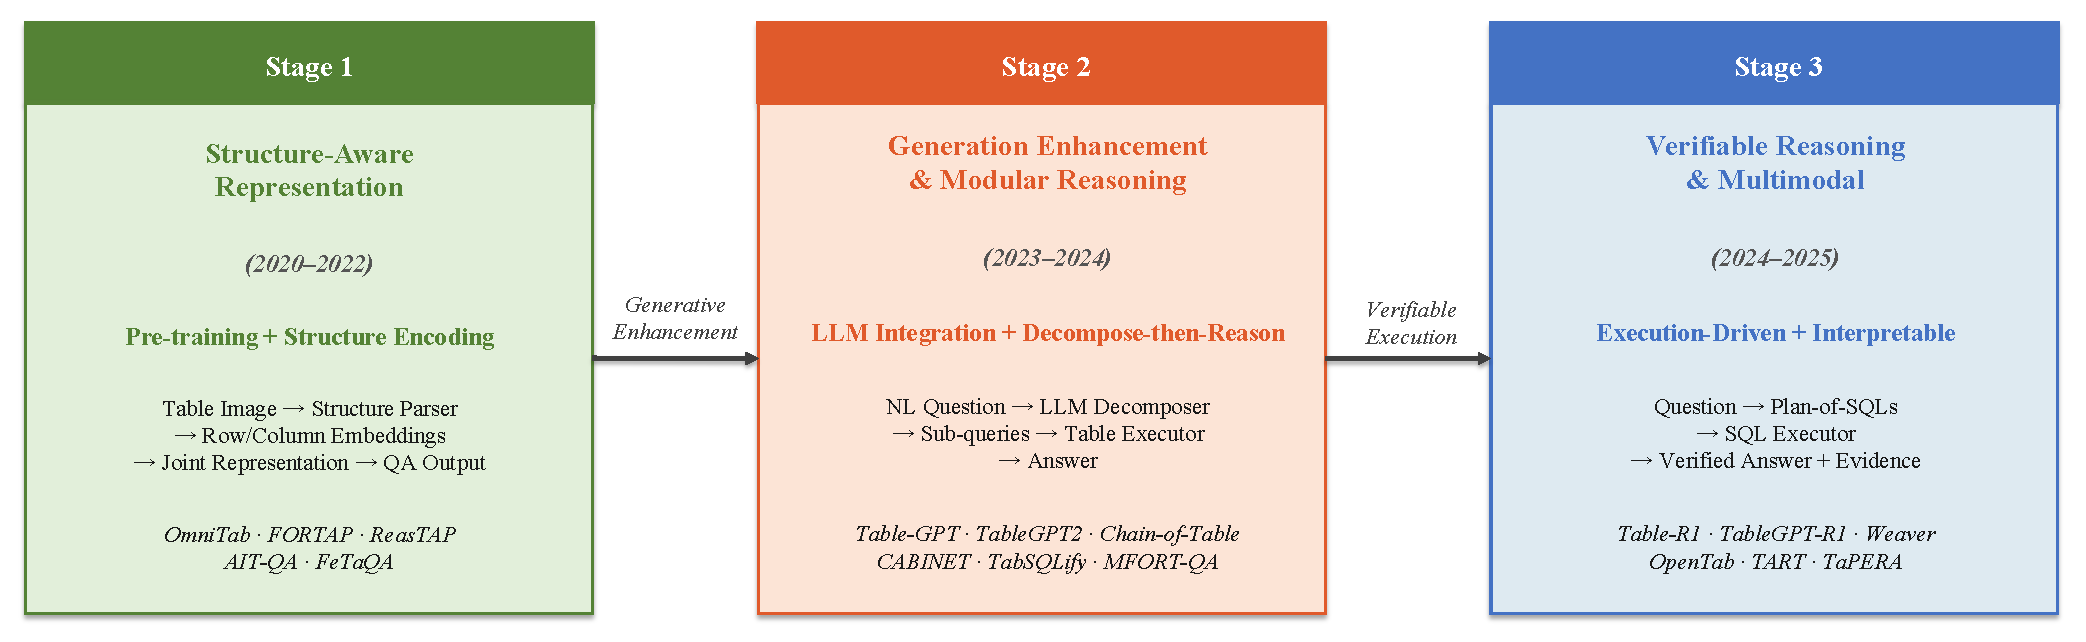
\includegraphics[width=0.95\textwidth]{figs/fig05.pdf}
\caption{Three-stage evolution of table understanding and question answering: Stage~1 establishes structure-aware representation learning; Stage~2 advances generation enhancement and modular reasoning; Stage~3 achieves verifiable reasoning and multimodal understanding.}
\label{fig:table_stages}
\end{figure*}


%%--------------------------------------------------------------------
%%  Section 4: Text-Based RAG
%%--------------------------------------------------------------------
\section{Text-Based Retrieval-Augmented Generation}
\label{sec:text_rag}

Document-level question answering faces two core challenges: LLMs are limited by context length for long or multi-document inputs, and pure generative models are prone to hallucinations without external evidence constraints.

\subsection{Retrieval-Augmented Generation}

Early RAG followed the classic ``retrieve-then-generate'' paradigm, improving DocQA performance through evidence recall quality and multi-hop support.

\subsection{Graph-Enhanced RAG}

Recent research has treated retrieval as a decision-making step directly driven by the reasoning process, utilizing graph structures for evidence organization.

\begin{figure*}[t]
\centering
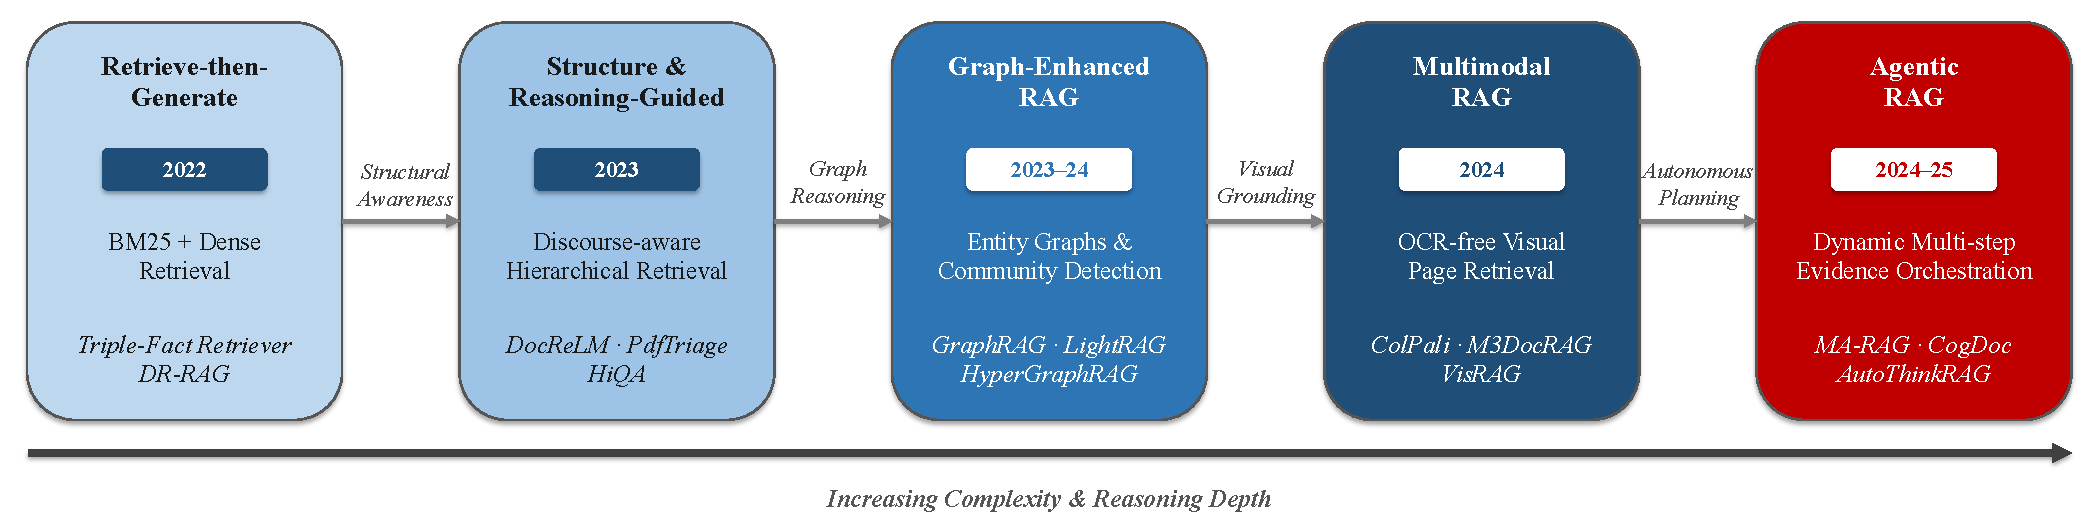
\includegraphics[width=0.95\textwidth]{figs/fig06.pdf}
\caption{Five-stage evolution of retrieval-augmented generation paradigms for document question answering.}
\label{fig:rag_evolution}
\end{figure*}


%%--------------------------------------------------------------------
%%  Section 5: Vision-Language Models
%%--------------------------------------------------------------------
\section{Vision-Language Models for Document Understanding}
\label{sec:vlm}

Vision-Language Models (VLMs) have propelled visual document understanding from single-modality analysis toward unified multimodal modeling. By jointly modeling visual content, textual semantics, and spatial layout information, VLMs enable deeper understanding of document structures.

\subsection{Foundational Vision-Language Models}

Early research established technical foundations for document image classification and cross-modal retrieval. The pre-training era brought multimodal integration with models such as LayoutXLM and VinVL.

\subsection{OCR-Free and Multi-Page Context}

Traditional document understanding relies on OCR to convert document images into text before semantic analysis. OCR-free models utilize joint vision-language modeling, taking raw document images as direct input.

\begin{figure*}[t]
\centering
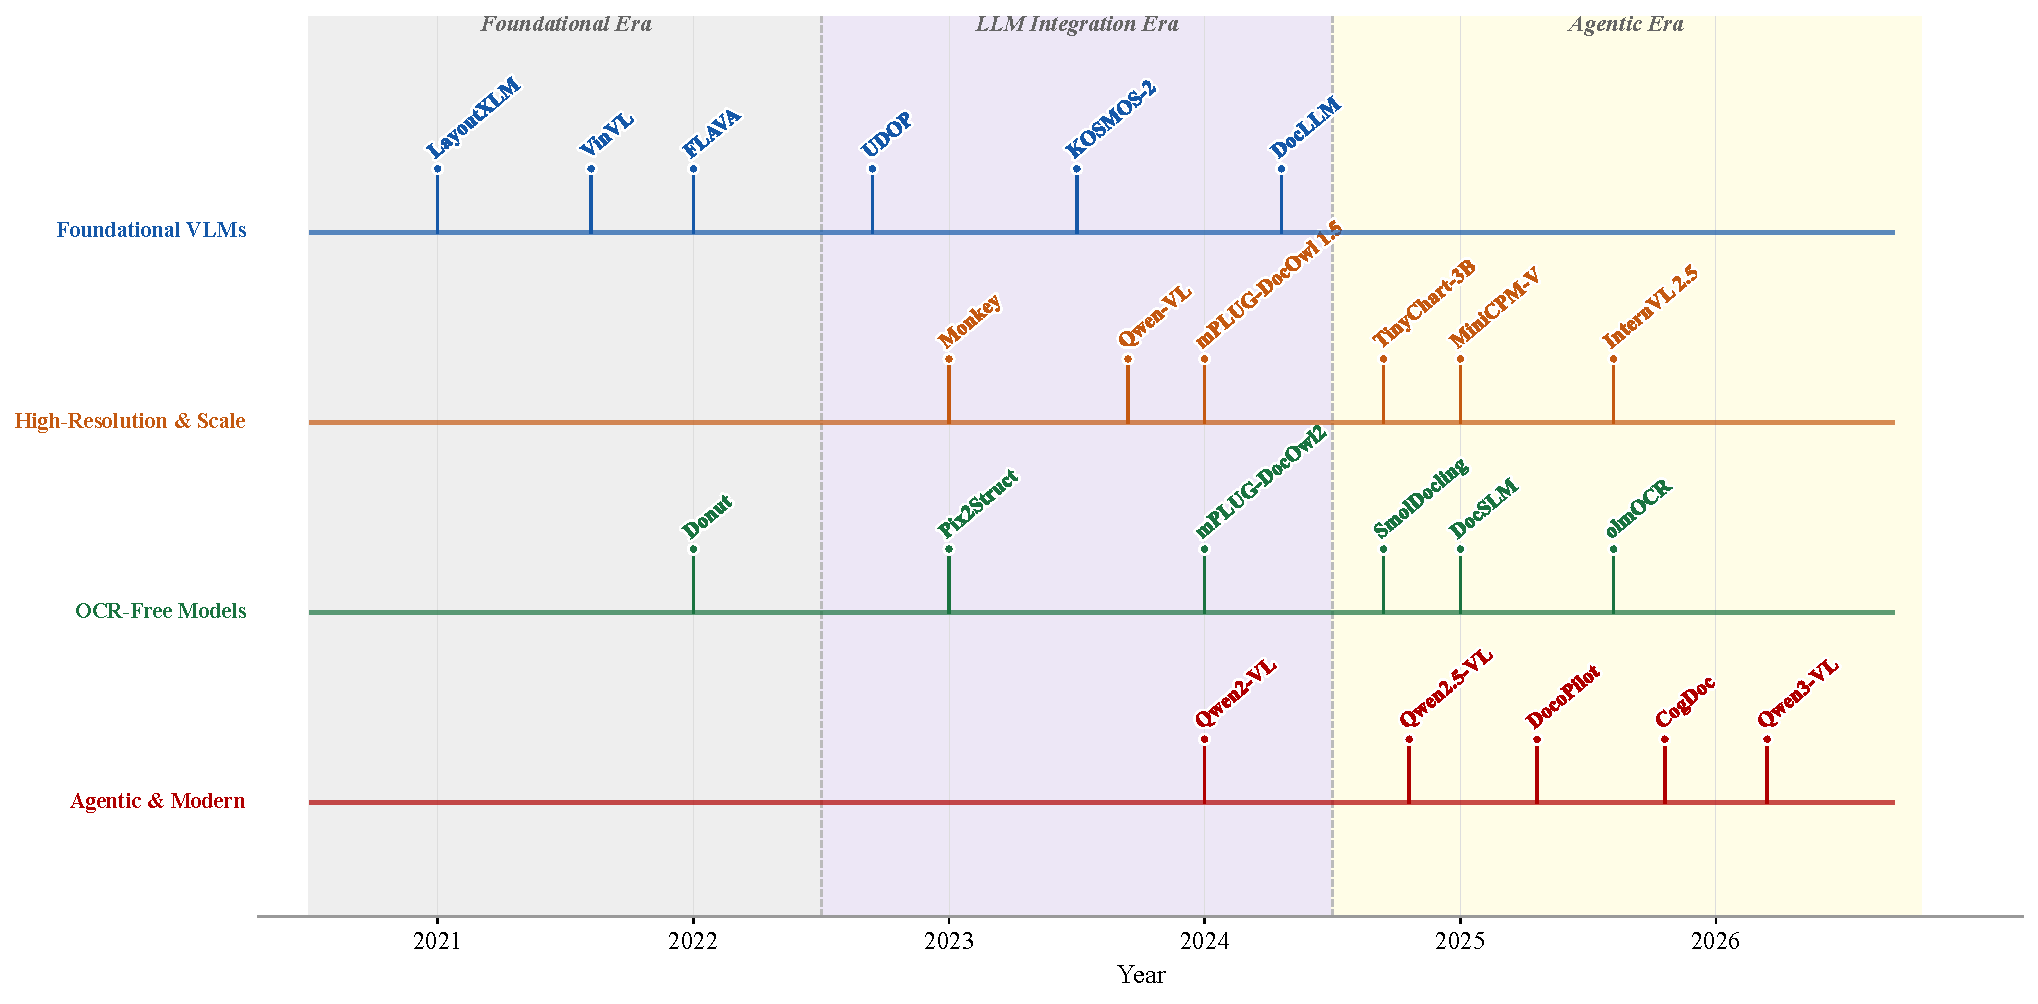
\includegraphics[width=0.95\textwidth]{figs/fig07.pdf}
\caption{Evolution of vision-language models for document understanding---organized into four development tracks: foundational vision-language models, high-resolution and scaled architectures, OCR-free models, and agentic systems.}
\label{fig:vlm_evolution}
\end{figure*}


%%--------------------------------------------------------------------
%%  Section 6: Evaluation
%%--------------------------------------------------------------------
\section{Evaluation}
\label{sec:eval}

With the advancement of Large Language Models, the performance of models in complex document processing and RAG tasks has become a central focus of research.

\subsection{Visual Document Understanding and Basic QA Evaluation}

Document Question Answering (DocQA) research focuses on whether models can correctly understand text, layout, and visual cues from single-page or small-scale documents.

\begin{figure*}[t]
\centering
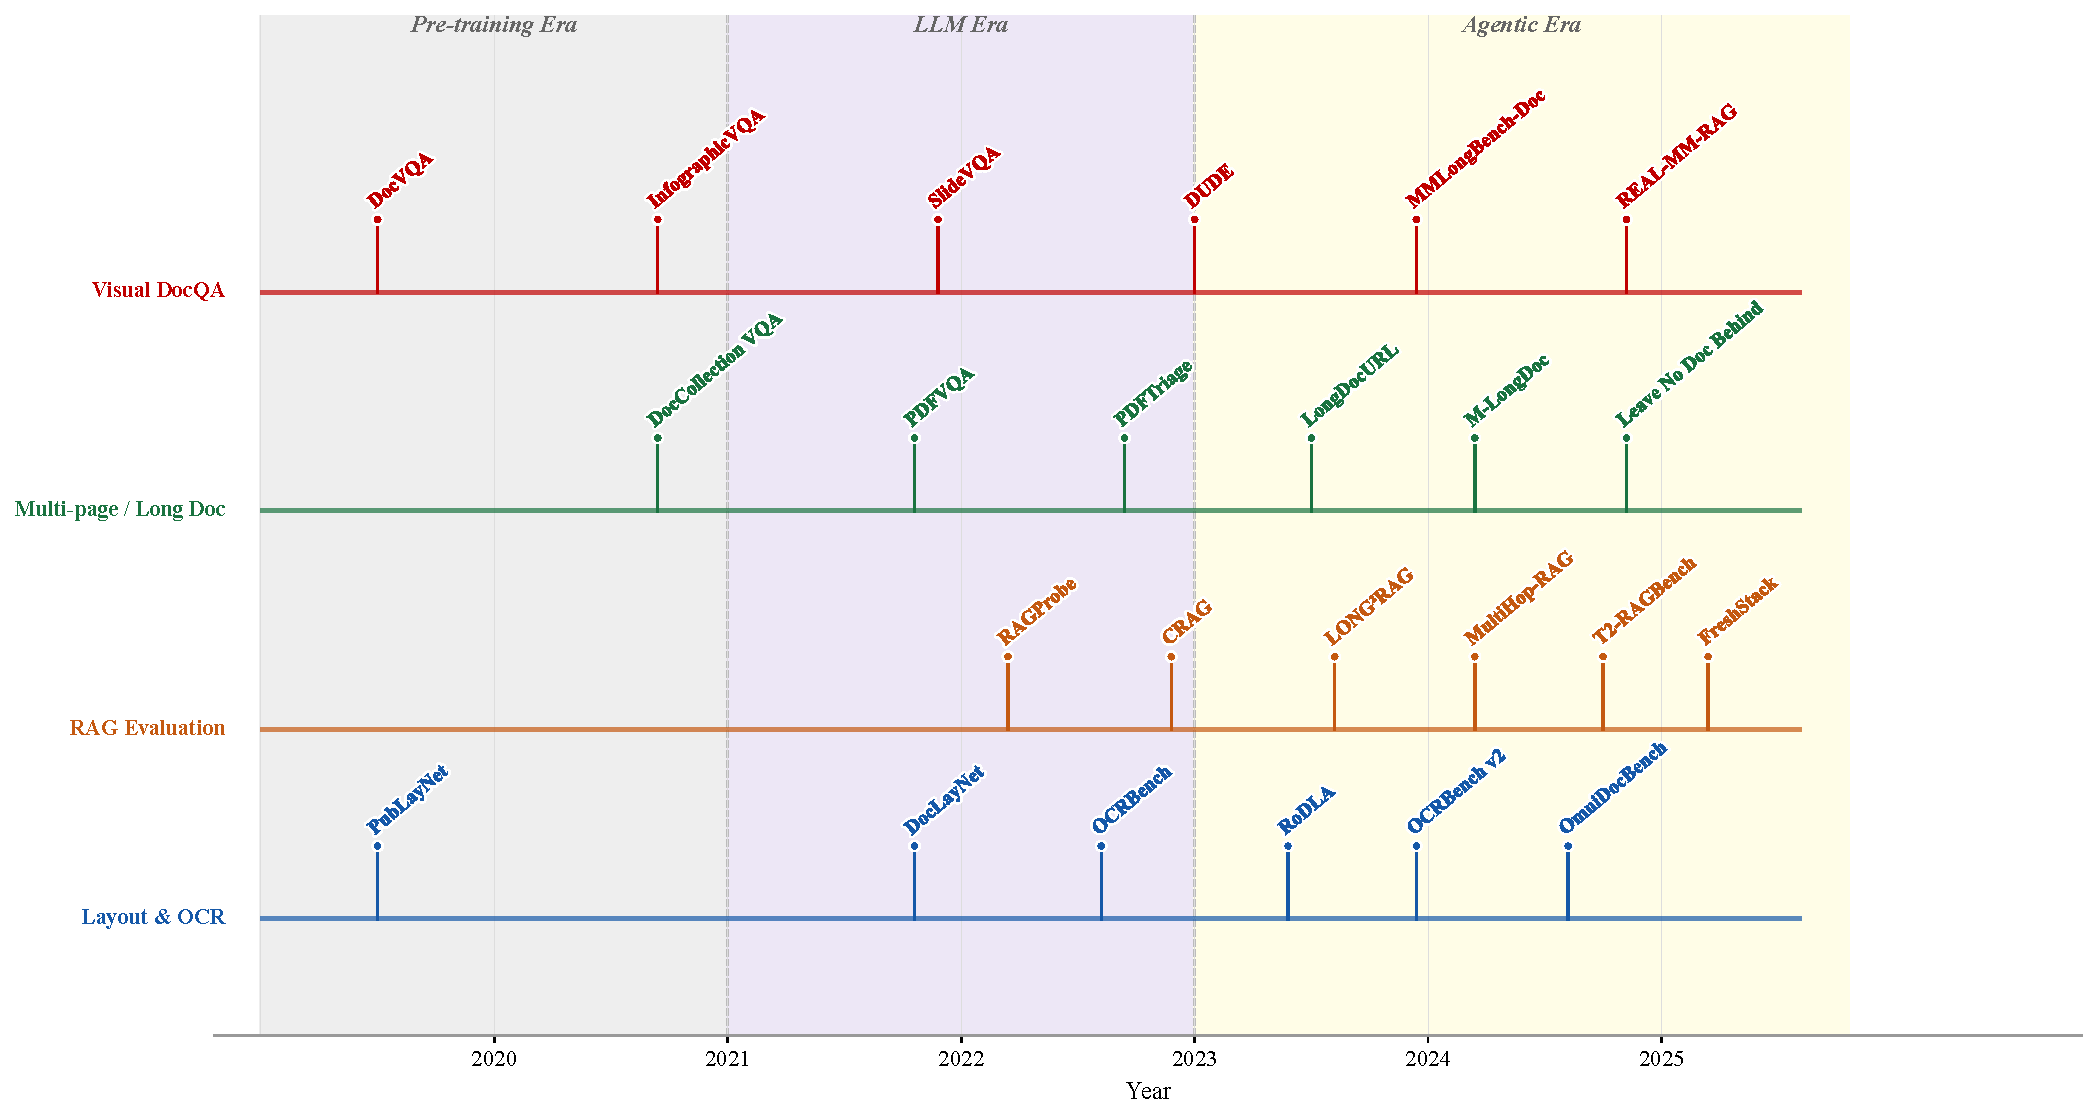
\includegraphics[width=0.95\textwidth]{figs/fig10.pdf}
\caption{Benchmark landscape for document intelligence (2019--2025): evaluation datasets organized into four categories.}
\label{fig:benchmarks}
\end{figure*}


%%--------------------------------------------------------------------
%%  Section 7: Conclusion
%%--------------------------------------------------------------------
\section{Future Research Directions and Conclusion}
\label{sec:conclusion}

Although document intelligence has evolved from OCR-centered pipeline approaches to end-to-end systems capable of cross-page, multimodal understanding and retrieval-augmented generation, achieving stable deployment in real-world scenarios still faces critical challenges.

\subsection{Verifiable and Structure-Aware Document Understanding}

Current document question answering systems can often produce seemingly plausible answers, yet these answers frequently lack explicit and verifiable evidence.

\subsection{Multimodal RAG and Agentic Systems}

As document understanding tasks extend from single pages to long documents and even collections of multiple documents, the system's challenge is no longer merely to find the page that contains the answer.

\subsection{Conclusion}

This survey has provided a comprehensive review of document intelligence research, tracing the evolution from traditional OCR and layout analysis through deep learning innovations to contemporary multimodal foundation models.


%%--------------------------------------------------------------------
%%  Bibliography
%%--------------------------------------------------------------------
\clearpage
\bibliographystyle{plainnat}
\setlength{\bibhang}{0pt}
\setlength\bibindent{0pt}
\bibliography{main}

\end{document}
